\documentclass[10pt,letterpaper]{article}
\usepackage[T1]{fontenc}
\usepackage{amsmath}
\usepackage{amssymb}
\usepackage{amsthm}
\usepackage{enumitem}
\usepackage[margin=0.5in]{geometry}
\usepackage{graphicx}
\usepackage{xcolor}

\definecolor{TangGreen}{HTML}{377459}

\title{Design and Analysis of Algorithms Homework 4}
\author{Jeremy Chen}
\begin{document}
	\maketitle
	
\subsection*{Problem 1.\hfill (25 points)}
\textbf{Ford-Fulkerson by hand and local updates.}

\begin{figure}[h!]
\centering
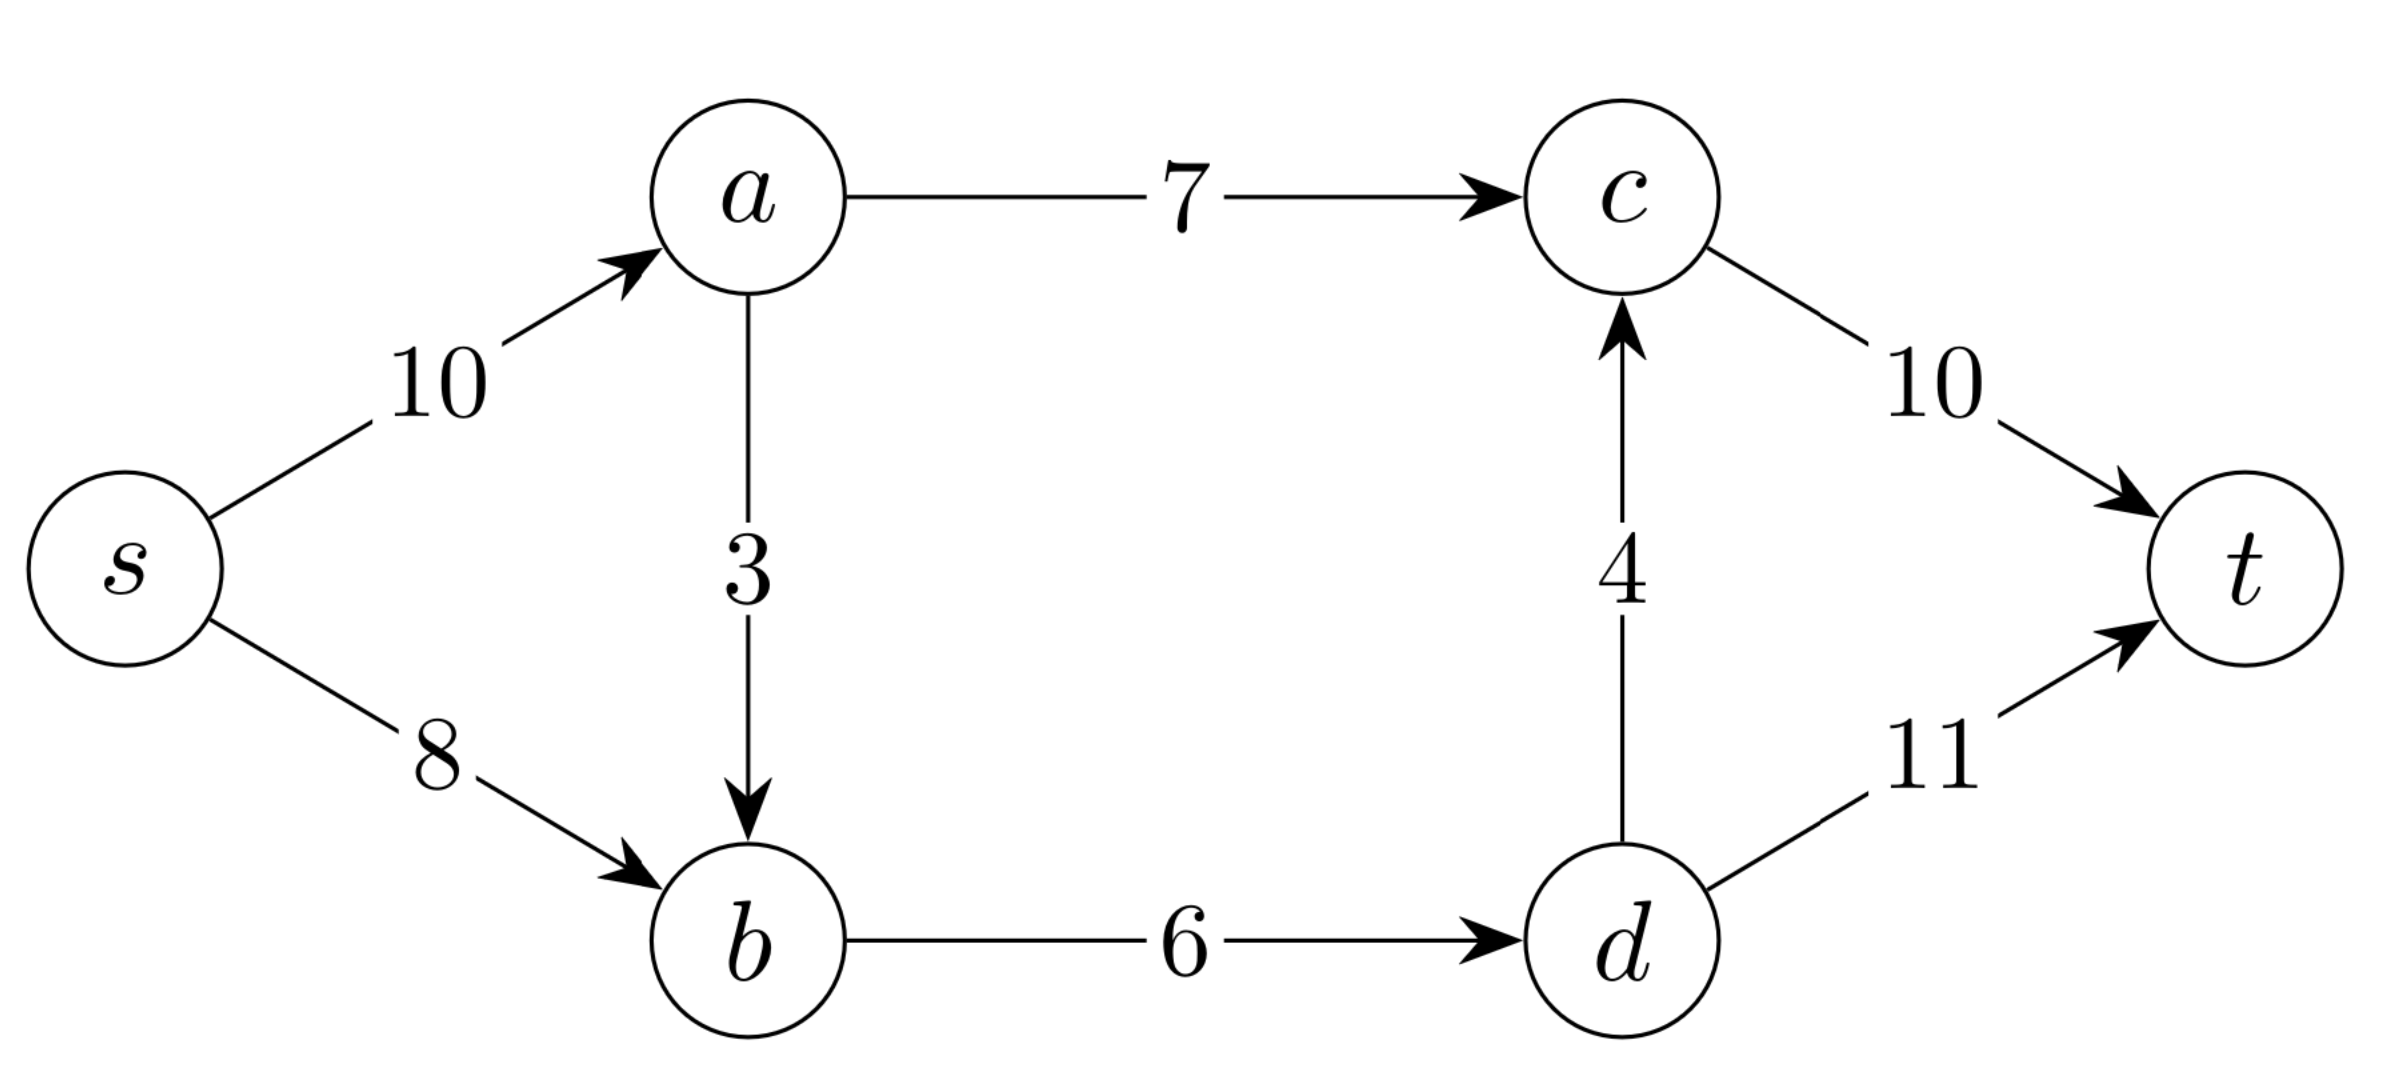
\includegraphics[width=0.5\linewidth]{fordfulkerson.png}
\end{figure}

\begin{enumerate}[label*=(\alph{enumi}), wide=0pt]

\item \textbf{(8 points)} Run Ford-Fulkerson on the network above, choosing any augmenting paths you like. List each augmenting path and its bottleneck. Report the value of the maximum flow and the flow on every edge. Then give a minimum cut $(s, V\ \backslash\ S)$, list the edges crossing it, and check that its capacity equals the value of your flow.

\color{TangGreen}
The first augmented path selected will be $s \rightarrow b \rightarrow d \rightarrow t$. The max flow is bottle-necked by $b \rightarrow d$, which has a capacity of 6. The second augmented path selected will be $s \rightarrow a \rightarrow c \rightarrow t$. The max flow is bottlenecked by $a \rightarrow c$, which has capacity 7. These are the only two augmented paths available, because in order for $s$ to reach $t$, it must go past either $a \rightarrow c$ or $b \rightarrow d$, and both of those edges have already reached maximum capacity. Therefore, the maximum flow is 13, with the following flow for edges
\begin{itemize}

\item $s \rightarrow a = 7$ 

\item $s \rightarrow b = 6$

\item $a \rightarrow c = 7$

\item $a \rightarrow b = 0$

\item $b \rightarrow d = 6$

\item $d \rightarrow c = 0$

\item $c \rightarrow t = 7$

\item $d \rightarrow t = 11$

\end{itemize}
The minimum cut disconnects $a \rightarrow c$ and $b \rightarrow d$, which has capacity of 13, matching the maximum flow. 
\color{black}

\item \textbf{(5 points)} Consider the network with edges $s \rightarrow u$, $s \rightarrow v$, $u \rightarrow t$, $v \rightarrow t$, each of capacity $C$, and an edge $u \rightarrow v$ of capacity 1. Show that Ford-Fulkerson, with a poor choice of augmenting paths, can take $2C$ augmentations, while Edmonds-Karp takes 2. Explain in one sentence why an $O(mC)$ bound is not polynomial in input size. 

\color{TangGreen}
If the augmentation chose to go through $u \rightarrow v$, updating that augmentation would require increasing $|f|$ by 1 for $2C$ times. Given that all capacities are $C$, and $|f*| \leq mC$, the bound is given by $O(m^{2}C)$. 
\color{black}

\item You are given a network $G$ with integer capacities and an integral maximum flow $f$ in it. The capacity of a single edge $e$ is now increased by 1. Give an $O(m + n)$-time algorithm that computes a maximum flow in the new network, and prove that it is correct.

\color{TangGreen}

\color{black}

\end{enumerate}

\subsection*{Problem 2.\hfill(25 points)}
\textbf{Understanding minimum cuts.} Throughout, $G$ is a directed simple graph (flow network) with source $s$, sink $t$, and positive capacities. 

\begin{enumerate}[label=(\alph{enumi}), wide=0pt]

\item \textbf{(5 points)} Prove or find a counterexample: if all edge capacities are distinct, then $G$ has a unique minimum $s$-$t$ cut. 

\color{TangGreen}
Given the following flow network, there are two distinct minimum $s$-$t$ cuts, one containing \{ $s \rightarrow u$, $v \rightarrow t$ \} and one containing \{ $s \rightarrow v$, $u \rightarrow t$ \}. 
\color{black}

\item \textbf{(5 points)} Prove or find a counterexample: if $(S, T)$ is a minimum cut of $G$, and we add 1 to the capacity of every edge, then $(S, T)$ is still a minimum cut. 

\end{enumerate}

\end{document}